% !TEX root = ../../../main.tex

\toggletrue{image}
\toggletrue{imagehover}
\chapterimage{logic_gates}
\chapterimagetitle{\uppercase{Logic Gates}}
\chapterimageurl{https://xkcd.com/2497/}
\chapterimagehover{In C, the multiocular O represents the bitwise norxondor gorgonax.}

\chapter{Halbaddierer}
\label{chapter-halbaddierer}

Ziel dieses und der folgenden Kapitel ist es, ein Schaltnetz zu konstruieren, das in der Lage ist, zwei mehrstellige Dualzahlen zu addieren. Die Lernziele dieses Kapitels sind:\\

\newcommand{\halbaddiererLernziele}{
\protect\begin{minipage}{\textwidth}
\begin{todolist}
\item Sie definieren, was ein Addiernetz ist.
\item Sie erstellen ein Schaltnetz, das zwei Binärziffern addieren kann.
\item Sie vereinfachen ein Schaltnetz, sodass es weniger Logikgatter benötigt.
\item Sie definieren, was ein Halbaddierer ist.
\end{todolist}
\end{minipage}
}

\lernziel{\autoref{chapter-halbaddierer}, \nameref{chapter-halbaddierer}}{\protect\halbaddiererLernziele}

\halbaddiererLernziele

\section{Addiernetz}

Ein Addiernetz automatisiert die schriftliche Addition zweier Dualzahlen im Computer.

\begin{definition}[Addiernetz]
Ein Addiernetz ist ein Schaltnetz, das zwei mehrstellige Dualzahlen addieren kann. Es ist Teil eines Prozessors, einer zentralen Hardware-Komponente eines Computers.
\end{definition}

Wir werden das Addiernetz schrittweise über mehrere Kapitel konstruieren. 

\section{Konstruktion des Halbaddierers}

Wir realisieren nun die Addition von \textbf{zwei} Binär\textbf{ziffern} durch ein Schaltnetz. Dies geschieht bei der schriftlichen Addition von zwei mehrstelligen Dualzahlen immer in der Spalte ganz rechts vor, wie das folgende Beispiel zeigt.

\begin{figure}[htb]
\centering
\begin{equation*}
\begin{tikzpicture}[
    row 3/.style={font=\scriptsize},
    every node/.style={column sep=.5mm, row sep=1mm}]
    \matrix (m) [matrix of math nodes,
        nodes in empty cells,
        %nodes=draw
    ] 
    {
    		& 	& 1 & 0 & 1 & \textbf{1} & [5mm]	\text{1. Summand} \\
	+      & 	&    & 1 & 1 & \textbf{1} &      	\text{2. Summand} \\ 
		& 1 	& 1 & 1 & 1 &    &         	\text{Überträge} \\
        		& 1 	& 0 & 0 & 1 & 0 &      	 \text{Summe} \\                                                  
    };
    \draw[-,color=black, semithick] (m-3-1.south west) -- (m-3-6.south east);
\end{tikzpicture}
\end{equation*}
\end{figure}

Das Schaltnetz muss in der Lage sein, alle vier Kombinationen von zwei Binärziffern zu addieren. Wir fassen die vier Kombinationen in \autoref{table-wahrheitstabelle-halbaddierer} zusammen und verwenden die in der Digitaltechnik üblichen Bezeichnungen. Wir können nun \autoref{table-wahrheitstabelle-halbaddierer} als Wahrheitstabelle auffassen und daraus mit den bekannten Werkzeugen ein Schaltnetz konstruieren.

\begin{table}[htb]
\centering
\begin{tblr}{|Q[c, m, 2cm]|Q[c, m, 2cm]||Q[c, m, 2cm]|Q[c, m, 2cm]|}
\hline
\SetCell[c=2]{c} Eingänge & & \SetCell[c=2]{c} Ausgänge \\ \hline
Bit $x$ & Bit $y$ & Summe $s$ & ausgehender Übertrag $c_{\text{out}}$ \\ \hline[2pt]
0 & 0 & 0 & 0 \\ \hline
0 & 1 & 1 & 0 \\ \hline
1 & 0 & 1 & 0 \\ \hline
1 & 1 & 0 & 1 \\ \hline
\end{tblr}
\caption{Der Übertrag wird als ausgehender Übertrag bezeichnet (engl. carry out), da bei der Addition am Ausgang ein Übertrag erzeugt wird.}
\label{table-wahrheitstabelle-halbaddierer}
\end{table}

\subsection{Übungen}

Lösen Sie die Übungen in der vorgegebenen Reihenfolge.

\begin{exercise}
\label{exercise-dnf-halbaddierer}
Erstellen Sie für die Wahrheitstabelle (siehe \autoref{table-wahrheitstabelle-halbaddierer}) eine boolesche Formel in \ac{DNF}. Sie müssen also für $s$ und $c_{\text{out}}$ \textbf{jeweils} eine boolesche Formel in \ac{DNF} erstellen.

\fillwithgrid{1in}
\end{exercise}

\begin{exercise}
\label{exercise-schaltnetz-halbaddierer}
Zeichen Sie für die booleschen Formeln aus Übung \ref{exercise-dnf-halbaddierer} das entsprechende Schaltnetz. Es handelt sich um \textbf{ein} Schaltnetz mit \textbf{zwei} Eingängen und \textbf{zwei Ausgängen}.

\fillwithgrid{2in}

\end{exercise}

\begin{exercise}
Zeichnen Sie in das Schaltnetz aus Übung \ref{exercise-schaltnetz-halbaddierer} ein, wie das Schaltnetz das Ergebnis von $x = 1$ und $y = 1$ berechnet. Tragen Sie dazu vor und nach jedem Logikgatter entweder $0$ oder $1$ ein. Tragen Sie abschliessend die korrekten Bits an den Ausgängen ein.
\end{exercise}

\newpage

\section{Der Halbaddierer}

Für die Wahrheitstabelle aus \autoref{table-wahrheitstabelle-halbaddierer} erhalten wir die Formeln $s = (\neg x \wedge y) \vee (x \wedge \neg y)$ und $c_{\text{out}} = x \wedge y$. Dies ergibt das in \autoref{half-adder-schaltnetz-1} dargestellte Schaltnetz.

\begin{figure}[ht]
\centering
\begin{circuitikz}
\draw (-2, 1) node[and port] (AND1) {};
\draw (-2, -1) node[and port] (AND2) {}; 
\draw (0, -2.5) node[and port] (AND3) {};

\draw (0,0) node[or port] (OR1) {}; 

\draw (-4,1.5) node[european not port] (NOT1) {};
\draw (-4,-1.5) node[european not port] (NOT2) {};

\draw (OR1.out) -+(1,0) node[anchor=west] {$s$};
\draw (AND3.out) -+(1,-2.5) node[anchor=west] {$c_{\text{out}}$};

\draw (-9, 0.5) node (x) {$x$};
\draw (-7, 0.5) node[circle, fill, inner sep=1pt] (xC1) {};
\draw (-7, -0.775) node[circle, fill, inner sep=1pt] (xC2) {};

\draw (-9, -0.25) node (y) {$y$};
\draw (-7.5, -0.25) node[circle, fill, inner sep=1pt] (yC1) {};
\draw (-7.5, -1.5) node[circle, fill, inner sep=1pt] (yC2) {};

\draw (AND1.out) |- (OR1.in 1);
\draw (AND2.out) |- (OR1.in 2);

\draw (NOT1.out) |- (AND1.in 1);
\draw (NOT2.out) |- (AND2.in 2);

\draw (x.east) |- (xC1);
\draw (xC1) |- (NOT1.in);
\draw (xC1) |- (AND2.in 1);
\draw (xC2) |- (AND3.in 1);

\draw (y.east) |- (yC1);
\draw (yC1) |- (NOT2.in);
\draw (yC1) |- (AND1.in 2);
\draw (yC2) |- (AND3.in 2);
\end{circuitikz}
\caption{Schaltnetz für einen Halbaddierer als \protect\say{White Box}).}
\label{half-adder-schaltnetz-1}
\end{figure}

Das Schaltnetz in \autoref{half-adder-schaltnetz-1} kann zwei Binärziffern addieren. Es ist somit ein Halbaddierer.

\begin{definition}[Halbaddierer]
Ein Schaltnetz, das zwei beliebige Binärziffern addieren kann, wird als \textbf{Halbaddierer} (engl. half adder, abgekürzt \acs{HA}) bezeichnet.
\end{definition}

Es gibt verschiedene Schaltnetze, die einen Halbaddierer (\ac{HA}) darstellen. Das Schaltnetz in \autoref{half-adder-schaltnetz-1} ist eine Möglichkeit der Realisierung. Unabhängig davon, wie wir das Schaltnetz für den Halbaddierer konstruieren, verwenden wir nun die Darstellung in \autoref{figure-ha-block} für den Halbaddierer. Es stellt ein eigenständiges Bauteil dar, das auch so gekauft werden kann. Wir können es uns so vorstellen, dass das Schaltnetz in \autoref{half-adder-schaltnetz-1} dahinter \say{versteckt} ist.

\begin{figure}[htb]
\centering
\begin{circuitikz}[american]
	\ctikzset{multipoles/dipchip/width=2}
	\draw (0,0) node[dipchip, num pins=4, hide numbers, no topmark] (HA1) {\textbf{\acs{HA}}};
	\node [right] at (HA1.bpin 1) {$x$};
	\node [right] at (HA1.bpin 2) {$y$};
	\node [left] at (HA1.bpin 4) {$s$};
	\node [left] at (HA1.bpin 3) {$c_{\text{out}}$};
\end{circuitikz}
\caption{Ein Halbaddierer als \protect\say{Black Box} mit zwei Eingängen ($x$ und $y$) und zwei Ausgängen ($s$ und $c_{\text{out}}$). Die Eingänge stellen zwei Binärziffern dar. Die Ausgänge zeigen die Summe und den ausgehenden Übertrag (engl. carry out, kurz $c_{\text{out}}$) an.}
\label{figure-ha-block}
\end{figure}

\begin{figure}[H]
\centering
\begin{minipage}{0.45\textwidth}
\centering
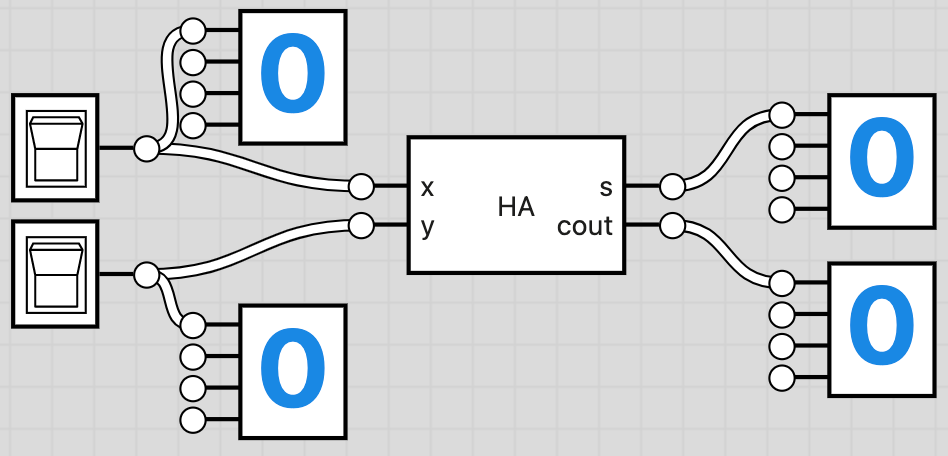
\includegraphics[width=\textwidth]{ha_1}
\end{minipage}
\begin{minipage}{0.45\textwidth}
\centering
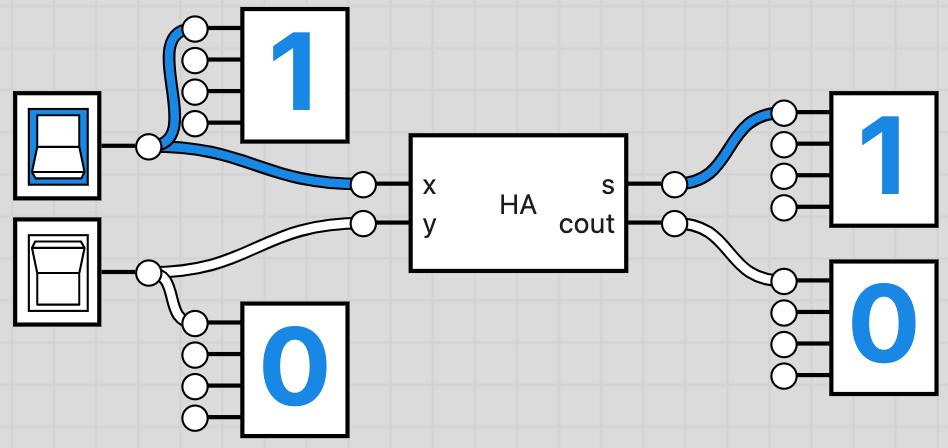
\includegraphics[width=\textwidth]{ha_2}
\end{minipage}
\begin{minipage}{0.45\textwidth}
\centering
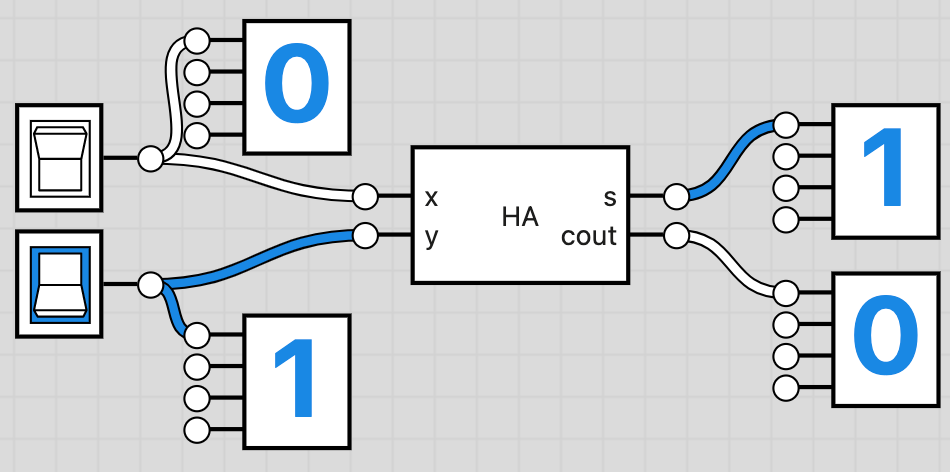
\includegraphics[width=\textwidth]{ha_3}
\end{minipage}
\begin{minipage}{0.45\textwidth}
\centering
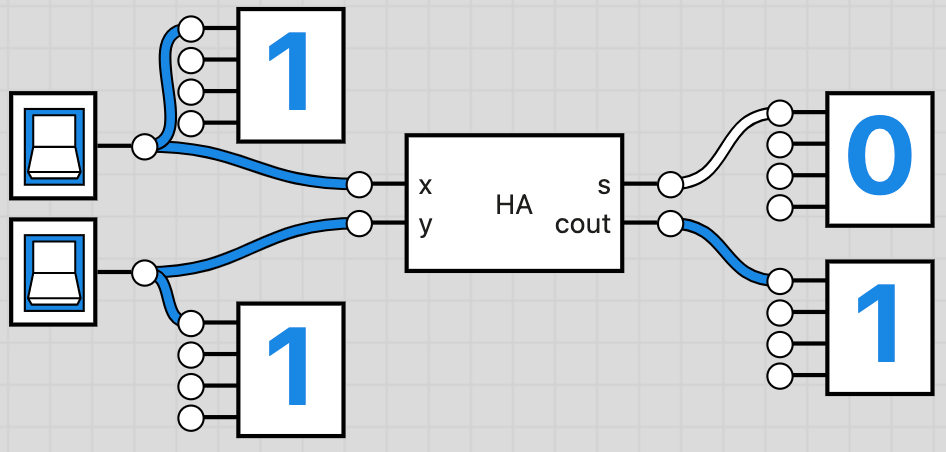
\includegraphics[width=\textwidth]{ha_4}
\end{minipage}
\caption{Der Halbaddierer simuliert in Logicly. Alle vier Kombinationen werden angezeigt.}
\end{figure}

\newpage

\subsection{Übungen}

Lösen Sie die Übungen in der vorgegebenen Reihenfolge.

\begin{exercise}
\label{exercise-ha-xor}
Ein Teil des Schaltnetzes für den Halbaddierer kann kompakter dargestellt werden. Vereinfachen Sie die Formel $s = (\neg x \wedge y) \vee (x \wedge \neg y)$ so, dass nur \textbf{ein boolescher Operator} verwendet wird. Sehen Sie sich dazu ggf. noch einmal Übung \ref{exercise-xor-nor-nand-xnor} an.
\fillwithgrid{0.5in}
\end{exercise}

\begin{exercise}
Zeichnen Sie erneut das Schaltnetz für einen Halbaddierer. Berücksichtigen Sie diesmal Ihre Ergebnisse aus Übung \ref{exercise-ha-xor}.
\fillwithgrid{2in}
\end{exercise}

\begin{exercise}
\begin{enumerate}
\item[a)] Notieren Sie eine schriftliche Addition von \textbf{zwei unterschiedlichen Dualzahlen} mit \textbf{je drei Bits}. Berechnen Sie das Ergebnis schriftlich.
\fillwithgrid{1in}
\item[b)] Markieren Sie die \textbf{Stelle}, welche mit einem \textbf{Halbaddierer} durchgeführt werden kann.
\item[c)] Warum kann man die anderen Stellen \textbf{nicht} mit einem Halbaddierer realisieren?
\fillwithgrid{\stretch{1}}
\end{enumerate}
\end{exercise}
